\chapter{Traveling Salesman Problem with Drone}

\section{Flying Sidekick Traveling Salesman Problem}
Flying Sidekick Traveling Salesman Problem (FSTSP) 由Murray(2015)等\cite{murrayFlyingSidekickTraveling2015}提出。FSTSP描述:假定有$c$个顾客需要服务,这个服务可以由无人机或者卡车来提供,但是有些顾客由于某些限制(比如包裹重量超过无人机的载重限制)只能由卡车提供服务。卡车和无人机必须从单一仓库出发,并且返回该仓库一次,即不能重复访问该仓库,无人机和卡车可以同时或者分别离开(返回)仓库。在无人机起飞前需要卡车司机装载包裹和更换电池的时间$s_L$,降落时需要给无人机装卸货物和充电的时间$s_R$。每次无人机的一次服务称为一次sortie,一次sortie分为三个节点$\langle i,j,k \rangle$,起飞点$i$可以是仓库也可以是顾客点,中间节点$j$是需要服务的顾客节点,节点$k$可以是仓库也可以是卡车所在的顾客节点,无人机在整个运输过程中可以进行多次sortie服务多个顾客,但是一次sortie的时间必须在无人机的续航时间内。FSTSP的目标是最小化服务所有顾客并且返回仓库(无人机和卡车都返回)的时间。

关键假设如下:
\begin{itemize}
    \item 无人机每次sortie的过程中只能服务一个顾客节点,但是在这期间卡车可以服务多个顾客节点。
    \item 无人机被假定为匀速飞行,如果无人机比卡车提前到达会合点则无人机不能在中途停下休息以节省电量。
    \item 无人机可以在降落点重新发射,但是无人机不能返回上一次的发射点。
    \item 无人机和卡车的会合点必须在顾客节点,而不能在中间的任何位置会合,并且卡车不会重新访问已经服务过的顾客节点来回收无人机。
    \item 无人机和卡车都不能访问除了仓库以外的非顾客节点(即只考虑简化过后的实际情况),并且无人机和卡车都不能重新访问已经服务过的顾客节点。
    \item 如果无人机返回仓库则不能再次进行服务,这是基于大多顾客节点都离仓库较远(大于无人机的续航里程)的假设,在无人机可以直接起飞服务顾客节点的假设下,PDSTSP会更加适合。
\end{itemize}

FSTSP数学模型的符号含义如表\ref{tab:fstsp-sign-meaning}所示。

\begin{table}[!htbp]
    \begin{threeparttable}
    \centering
    \caption{FSTSP模型符号及含义}
    \label{tab:fstsp-sign-meaning}
    \begin{tabularx}{\textwidth}{lX}
        \toprule[1pt] % 表头线宽1镑(point, pt)
        符号 & 含义 \\
        \midrule[0.75pt] % 表中间线宽0.75镑(point, pt)
        $0$ & 起点仓库 \\
        $c + 1$ & 终点仓库(和起点仓库相同,只是为了建模方便的另一个记号) \\
        $C=\{1,2,\cdots,c\}$ & 全部客户集合 \\
        $C' \subseteq C$ & 无人机可访问的客户集合 \\
        $N_0 = \{0,1,2,\cdots,c\}$ & 流出节点集合 \\
        $N_+ = \{1,2,\cdots,c + 1\}$ & 流入节点集合 \\
        $N = \{0,1,2,\cdots,c,c + 1\}$ & 全部节点集合 \\
        \makecell[l]{$\langle i,j,k\rangle \in P,i \in N_0, j \in\{ C': j \neq i\},$\\
        $k \in\{ N_+: k \neq i, k \neq j,\tau_{ij}'+\tau_{jk}'\leq e\}$} & 无人机飞行路径集合 \\
        $\tau_{ij}'/\tau_{ij}, i \in N_0, j \in N_+, i \neq j, \tau_{0, c+1}\equiv 0\hyperlink{tab:fstsp-item-1}{\tnote{a}}$ & 弧$\langle i,j\rangle$的飞行/行驶时间成本 \\
        $s_L/s_R$ & 无人机发射/回收耗时 \\
        $e$ & 无人机续航时长,以单位时间来衡量 \\
        $x_{ij} \in \{0,1\}, i \in N_0, j \in N_+, i\neq j$ & 卡车路由决策变量 \\
        $y_{ijk} \in \{0,1\}, i \in N_0, j \in C, k\in \{N_+: \langle i,j,k \rangle \in P\}$ & 无人机路由决策变量 \\
        $t_i'/t_i\geq 0, i\in N_+, t_0' = t_0 = 0$ & 无人机/卡车有效到达时间戳辅助变量 \\
        $p_{ij} \in \{0,1\}\hyperlink{tab:fstsp-item-2}{\tnote{b}},p_{0j} = 1 ,\forall j \in C$ & 卡车访问次序先后辅助变量(为了确保无人机连续的sortie和卡车访问的顺序一致\hyperlink{tab:fstsp-item-3}{\tnote{c}}) \\
        $1 \leq u_i \leq c + 2, i \in N_+$ & 卡车破子圈辅助变量(和标准TSP的MTZ形式破子圈辅助变量类似\hyperlink{tab:fstsp-item-4}{\tnote{d}}) \\
        \bottomrule[1pt] % 表尾线宽1镑(point, pt)
    \end{tabularx}
    \begin{tablenotes}
        \footnotesize % 设置脚注内容字体大小为\footnotesize
        \item[a] \hypertarget{tab:fstsp-item-1}{}出于完备性的考虑,当只有一个顾客节点的时候,这个顾客将由无人机从仓库直接起飞进行服务。
        \item[b] \hypertarget{tab:fstsp-item-2}{}当卡车访问顾客节点$j\in \{C:j\neq i\}$时,顾客节点$i \in C$已经在之前的某个时间点被卡车访问过了,则$p_{ij} = 1$。
        \item[c] \hypertarget{tab:fstsp-item-3}{}当顾客节点$i$或者$j$仅被无人机服务时,$p_{ij}$的取值就不重要。
        \item[d] \hypertarget{tab:fstsp-item-4}{}$u_i$表示顾客点$i$在卡车访问的路径中的次序,比如$u_5 = 1$表示顾客点$i = 5$是卡车访问路径中的第1个节点,但是不同于TSP,在FSTSP中需要通过约束将无人机服务的顾客点$i$排除在外。
    \end{tablenotes}
    \end{threeparttable}
\end{table}

FSTSP数学模型可以表示为MILP \ref{model:model-fstsp}。

{
\newcommand{\mySubstack}[1]{\mathclap{\substack{#1}}}
\newcommand{\myYellowTag}[1]{\label{#1}\tag{\colorbox{shallow-yellow}{\theequation}}\addtocounter{equation}{1}}
\newcommand{\myRedTag}[1]{\label{#1}\tag{\colorbox{shallow-red}{\theequation}}\addtocounter{equation}{1}}
\newcommand{\myGreenTag}[1]{\label{#1}\tag{\colorbox{shallow-green}{\theequation}}\addtocounter{equation}{1}}
\newcommand{\myPurpleTag}[1]{\label{#1}\tag{\colorbox{shallow-purple}{\theequation}}\addtocounter{equation}{1}}

\begin{model}{FSTSP MILP}{model-fstsp}
\begin{align}
    \min \quad & t_{c + 1}  \label{eq:fstsp-obj}\\
    \text{s.t.} \quad & 
        \sum_{\substack{i\in N_{0}\\i\neq j}}x_{ij}+\sum_{\substack{i\in N_{0}\\ i\neq j}}\!\sum_{\substack{k \in N_{+}\\ \langle i,j,k \rangle \in P}}y_{ijk}=1, \quad \forall j \in C\myGreenTag{eq:fstsp-customer-visit}\\
    \quad & 
        \sum_{j\in N_{+}}x_{0j}=1\myPurpleTag{eq:fstsp-truck-start}\\
    \quad & 
        \sum_{i\in N_{0}}x_{i,c + 1}=1\myPurpleTag{eq:fstsp-truck-return}\\
    \quad & 
        u_i - u_j + 1 \leq (c + 2)(1 - x_{ij}), \quad \forall i \in C, j \in \{N_{+}:j \neq i\}\myPurpleTag{eq:fstsp-truck-mtz}\\
    \quad & 
        \sum_{\substack{i\in N_{0}\\ i \neq j}}x_{ij}=\sum_{\substack{k\in N_{+}\\k\neq j}}x_{jk}, \quad \forall j \in C\myPurpleTag{eq:fstsp-truck-continuity}\\
    \quad & 
        \sum_{\substack{j\in C\\j \neq i}}\!\sum_{\substack{k\in N_{+}\\\langle i,j,k \rangle\in P}}y_{ijk}\leq1, \quad \forall i\in N_{0}\myRedTag{eq:fstsp-drone-land}\\
    \quad & 
        \sum_{\substack{i\in N_{0}\\i\neq k}}\!\sum_{\substack{j\in C\\\langle i,j,k \rangle\in P}}y_{ijk}\leq1, \quad \forall k \in N_{+}\myRedTag{eq:fstsp-drone-takeoff}\\
    \quad & 
        2 y_{ijk} \leq \sum_{\substack{h \in N_0 \\ h \neq i}}x_{hi} + \sum_{\substack{l \in C\\ l \neq k}}x_{lk}, \quad \forall i \in C, j \in \{C: j \neq i\}, k \in \{N_{+}: \langle i,j,k \rangle \in P\}\myYellowTag{eq:fstsp-drone-truck-meet}\\
    \quad & 
        y_{0jk} \leq \sum_{\substack{h \in N_0 \\ h \neq k}}x_{hk}, \quad \forall j \in C, k \in \{N_{+}: \langle 0,j,k \rangle \in P\}\myYellowTag{eq:fstsp-drone-truck-meet-begin}\\
    \quad & 
        u_k - u_i \geq 1 - (c+2)\left(1 - \sum_{\mySubstack{j \in C \\ \langle i,j,k \rangle \in P}}y_{ijk}\right), \quad \forall i \in C, k \in \{N_{+}: k \neq i\}\myYellowTag{eq:fstsp-truck-visit-order}\\
    \quad & 
        t_i' \geq t_i - M\left(1 - \sum_{\substack{j \in C\\ j \neq i}}\sum_{\substack{k \in N_{+}\\ \langle i,j,k \rangle \in P}}y_{ijk}\right), \quad \forall i \in C\myYellowTag{eq:fstsp-truck-drone-takeoff-time-1}\\
    \quad & 
        t_i' \leq t_i + M\left(1 - \sum_{\substack{j \in C\\ j \neq i}}\sum_{\substack{k \in N_{+}\\ \langle i,j,k \rangle \in P}}y_{ijk}\right), \quad \forall i \in C\myYellowTag{eq:fstsp-truck-drone-takeoff-time-2}\\
    \quad & 
        t_k' \geq t_k - M\left(1 - \sum_{\substack{i \in N_0\\ i \neq k}}\sum_{\substack{j \in C\\ \langle i,j,k \rangle \in P}}y_{ijk}\right), \quad \forall k \in N_{+}\myYellowTag{eq:fstsp-truck-drone-land-time-1}\\
    \quad & 
        t_k' \leq t_k + M\left(1 - \sum_{\substack{i \in N_0\\ i \neq k}}\sum_{\substack{j \in C\\ \langle i,j,k \rangle \in P}}y_{ijk}\right), \quad \forall k \in N_{+}\myYellowTag{eq:fstsp-truck-drone-land-time-2}\\
    \quad & 
    \begin{aligned}
        &
            t_k \geq t_h + \tau_{hk} + s_{L}\left(\sum_{\substack{l \in C\\ l \neq k}}\sum_{\substack{m \in N_{+}\\ \langle k,l,m \rangle \in P}}y_{klm}\right) + s_{R}\left(\sum_{\substack{i \in N_0\\ i \neq k}}\sum_{\substack{j \in C\\ \langle i,j,k \rangle \in P}}y_{ijk}\right) - M(1 - x_{hk}), \\
        &\quad
            \forall h \in N_0, k \in \{N_{+}: k \neq h\}\\
    \end{aligned}\myYellowTag{eq:fstsp-truck-time}\\
    \quad & 
        t_{j}'\geq t_{i}'+\tau_{ij}'-M\left(1 - \sum_{\mySubstack{k \in N_{+}\\ \langle i,j,k \rangle \in P}}y_{ijk}\right), \quad \forall j\in C', i \in \{N_0: i \neq j\}\myRedTag{eq:fstsp-drone-time-fly}\\
    \quad &
        t_{k}'\geq t_{j}'+\tau_{jk}'+s_{R}-M\left(1-\sum_{\mySubstack{i\in N_{0}\\ \langle i,j,k\rangle \in P}}y_{ijk}\right), \quad \forall j\in C', k\in \{N_{+}: k \neq j\}\myRedTag{eq:fstsp-drone-time-fly-back}\\
    \quad & 
        t_k' - (t_j' - \tau_{ij}') \leq e + M(1 - y_{ijk}), \quad \forall k \in N_{+}, j \in \{C: j\neq k\}, i \in \{N_0: \langle i,j,k \rangle \in P\}\myRedTag{eq:fstsp-drone-endurance}\\
    \quad & u_i - u_j \geq 1 - (c+2)p_{ij}, \quad \forall i \in C, j \in \{C: j \neq i\}\label{eq:fstsp-drone-truck-aide-1}\\
    \quad & u_i - u_j \leq -1 + (c+2)(1 - p_{ij}), \quad \forall i \in C, j \in \{C: j \neq i\}\label{eq:fstsp-drone-truck-aide-2}\\
    \quad & p_{ij} + p_{ji} = 1, \quad \forall i \in C, j \in \{C: j \neq i\}\label{eq:fstsp-drone-order}\\
    \quad &
    \begin{aligned}
        &
            t_l' \geq t_k' - M\left(3 - \sum_{\mySubstack{j \in C\\ \langle i,j,k \rangle \in P\\ j \neq l}}y_{ijk} - \sum_{\substack{m \in C \\ m \neq i\\ m \neq k \\ m \neq l}}\sum_{\substack{n \in N_{+}\\ \langle l,m,n\rangle \in P\\ n \neq i\\ n\neq k}}y_{lmn}-p_{il}\right)\\
        &\quad
            \forall i \in N_0, k \in \{N_{+}: k \neq i\}, l \in \{C: l\neq i, l\neq k\}
    \end{aligned}\myRedTag{eq:fstsp-drone-sortie-order}\\
    \quad & t_0 = 0\label{eq:fstsp-truck-start-time}\\
    \quad & t_0'= 0\label{eq:fstsp-drone-start-time}\\
    \quad & p_{0j} = 1, \quad \forall j \in C\label{eq:fstsp-drone-start-order}\\
    \quad & x_{ij} \in \{0, 1\}, \quad \forall i \in N_0, j \in \{N_{+}:j \neq i\}\label{eq:fstsp-x-bound}\\
    \quad & y_{ijk} \in \{0, 1\}, \quad \forall i \in N_0, j \in \{C:j \neq i\}, k \in \{N_{+}:\langle i,j,k \rangle \in P\}\label{eq:fstsp-y-bound}\\
    \quad & 1 \leq u_i \leq c+2, \quad \forall i \in N_{+}\label{eq:fstsp-u-bound}\\
    \quad & t_i \geq 0, \quad \forall i \in N\label{eq:fstsp-truck-time-bound}\\
    \quad & t_i' \geq 0, \quad \forall i \in N\label{eq:fstsp-drone-time-bound}\\
    \quad & p_{ij}\in \{0, 1\}, \quad \forall i \in N_0, j \in \{C: j \neq i\}\label{eq:fstsp-drone-order-bound}
\end{align}
\end{model}
}

目标函数\ref{eq:fstsp-obj}追求最小化卡车到达终点仓库$c+1$的有效时间$t_{c+1}$,通过约束\ref{eq:fstsp-truck-drone-land-time-1}和\ref{eq:fstsp-truck-drone-land-time-2}来对齐无人机和卡车最晚到达终点仓库的时间,所以目标函数相当于$\min\{\max\{t_{c+1},t_{c+1}'\}\}$。

约束条件可以分为四类\cite{zhihu-murray2015}:

\begin{itemize}
    \item \colorbox{shallow-green}{客户有关的约束:}约束\ref{eq:fstsp-customer-visit}要求对于任何一位顾客$j$,必须且只能被卡车(或无人机)服务一次。
    \item \colorbox{shallow-purple}{卡车有关的约束:}
    \begin{itemize}
        \item 卡车流平衡约束:约束\ref{eq:fstsp-truck-start}要求卡车必须从起点仓库流出一次,约束\ref{eq:fstsp-truck-return}要求卡车必须从终点仓库流入一次,约束\ref{eq:fstsp-truck-continuity}要求卡车在中间节点满足流入和流出相等的流平衡约束。
        \item 卡车破子圈约束:约束\ref{eq:fstsp-truck-mtz}是MTZ形式的破子圈约束\cite{YunChouorWeiWoYouHuaQianTanLuXingShangWenTiTSPDeQiZhongZhengShuGuiHuaMoXing2022, YunChouorWeiWoYouHua|TSPZhongLiangZhongBuTongXiaoChuZiHuanLuDeFangFaJicallbackShiXianPythonDiaoYongGurobiQiuJie2020},去除了子圈存在的可能,这里$M$取到了$u_i - u_j + 1$的上界$c+2$,$u_i$可以理解为点$i$的访问次序,比如$u_1 = 5$可以理解为点1是从出发点开始,第五个被访问到的点。
    \end{itemize}
    \item \colorbox{shallow-red}{无人机有关的约束:}
    \begin{itemize}
        \item 无人机发射、回收节点流约束:约束\ref{eq:fstsp-drone-land}表示无人机可以从非终点仓库流出,约束\ref{eq:fstsp-drone-takeoff}表示无人机可以从非起点仓库流入。
        \item 无人机访问、回收节点时间戳约束:约束\ref{eq:fstsp-drone-time-fly}表示无人机访问顾客的时间戳应该符合时间逻辑,即不早于起飞时间戳$t_i'$+前往服务顾客点的飞行时长$\tau_{ij}'$\footnote{起飞时间$s_L$没有被包含进来的原因是,当无人机从顾客点$i$起飞时,约束\ref{eq:fstsp-truck-drone-takeoff-time-1}和\ref{eq:fstsp-truck-drone-takeoff-time-2}会使得$t_i' = t_i$,然后约束\ref{eq:fstsp-truck-drone-land-time-1}和\ref{eq:fstsp-truck-drone-land-time-2}会将起飞的时间$s_L$包含在飞行到顾客点$j$的时间内。},约束\ref{eq:fstsp-drone-time-fly-back}表示无人机回到卡车的时间戳应该符合时间逻辑,即不早于访问顾客点的$t_j'$+返回卡车的飞行时长$\tau_{jk}'$+回收无人机用时$s_R$\footnote{这里降落的时间$s_R$必须被包含进来的原因是,卡车可能比无人机更快到达会合点$k$(原文中举出了一个例子以助于理解\cite{murrayFlyingSidekickTraveling2015})。}。
        \item 无人机电量续航约束:约束\ref{eq:fstsp-drone-endurance}表示无人机的飞行时间不能超过其续航时间,即到达会合点$t_k'$的有效时间$-$无人机从节点$i$的起飞时间$(t_j'-\tau_{ij}')$(不直接使用$t_i'$是因为$t_i'$不是起飞的时间戳而是无人机到达$i$点的时间戳)要在无人机的续航时间$e$之内。
        \item 无人机飞行次序约束:约束\ref{eq:fstsp-drone-sortie-order}要求无人机对于任意两条路径$\langle i,j,k \rangle$和$\langle l,m,n \rangle$而言,如果无人机先从节点$i$起飞之后的某个时间才从节点$l$($p_{il}=1$)起飞,则无人机必须先完成上一次飞行才能继续下一次飞行($t_l'\geq t_k'$),并且任意两条路径之间无交叉。
    \end{itemize}
    \item \colorbox{shallow-yellow}{无人机和卡车同步有关的约束:}
    \begin{itemize}
        \item 无人机发射、回收点卡车访问约束:约束\ref{eq:fstsp-drone-truck-meet}要求对于非起点发射的无人机($\forall i \in C$),卡车必须经过无人机的起飞点$i$和降落点$k$,约束\ref{eq:fstsp-drone-truck-meet-begin}要求对于从起点仓库起飞的无人机来说,卡车必须经过无人机的降落点。
        \item 无人机访问顾客时卡车访问次序约束:约束\ref{eq:fstsp-truck-visit-order}要求卡车必须先访问无人机的起飞点再访问无人机的降落点。
        \item 无人机发射点时间戳约束:约束\ref{eq:fstsp-truck-drone-takeoff-time-1}和\ref{eq:fstsp-truck-drone-takeoff-time-2}为无人机发射点的有效时间约束,要求无人机在发射节点的有效时间等于卡车在该点的有效时间,共同实现了卡车和无人机在发射节点时间上的对齐。
        \item 无人机回收点时间戳约束:约束\ref{eq:fstsp-truck-drone-land-time-1}和\ref{eq:fstsp-truck-drone-land-time-2}为无人机回收点的有效时间约束,要求无人机在回收节点的有效时间等于卡车在该点的有效时间,共同实现了卡车和无人机在回收节点时间上的对齐。
        \item 卡车访问顾客节点时间戳约束:约束\ref{eq:fstsp-truck-time}要求卡车访问当前顾客点$k$时必须要先将需要起飞的无人机$s_L$发射或者需要降落的无人机$s_R$回收,并且要大于到达顾客点$h$的有效时间戳$t_h$+路径$\langle h,k \rangle$所花费的时间$\tau_{hk}$\footnote{这里假设卡车从$h \in N_0$行驶到$k \in N_+$。}。
    \end{itemize}
    \item 辅助变量和决策变量:
    \begin{itemize}
        \item 卡车访问次序约束:约束\ref{eq:fstsp-drone-truck-aide-1},\ref{eq:fstsp-drone-truck-aide-2}和\ref{eq:fstsp-drone-order}决定了卡车访问次序$p_{ij}$取值的合理性,$u_i$和$p_{ij}$主要用于约束被卡车访问的节点之间的次序,对于被无人机服务的顾客点$i$或者$j$来说,$u_i$和$p_{ij}$的取值并不重要。
        \item 辅助变量及决策变量的初始值和取值范围:约束\ref{eq:fstsp-truck-start-time}和\ref{eq:fstsp-drone-start-time}给定了卡车和无人机有效时间的初始值,约束\ref{eq:fstsp-drone-start-order}规定了起点仓库的访问次序一定在其他所有顾客节点之前,约束\ref{eq:fstsp-x-bound}和\ref{eq:fstsp-y-bound}给定了决策变量的取值范围,约束\ref{eq:fstsp-u-bound}规定了卡车破子圈辅助变量的取值范围,约束\ref{eq:fstsp-truck-time-bound}和\ref{eq:fstsp-drone-time-bound}规定了卡车和无人机的有效时间必须是非负实数,约束\ref{eq:fstsp-drone-order-bound}给定了卡车访问次序辅助变量的取值范围。
    \end{itemize}
\end{itemize}

在约束\cref{eq:fstsp-truck-drone-takeoff-time-1,eq:fstsp-truck-drone-takeoff-time-2,eq:fstsp-truck-drone-land-time-1,eq:fstsp-truck-drone-land-time-2,eq:fstsp-truck-time,eq:fstsp-drone-time-fly,eq:fstsp-drone-time-fly-back,eq:fstsp-drone-endurance}中,$M\geq \max\{t_{c+1}, t_{c+1}'\}$取一个非常大的数,需要大于等于最后到达终点仓库的卡车(无人机)的有效时间。由于无法事先确定最小可接受的$M$值,因此一种方法是用nearest neighbor heuristic来计算一个访问所有顾客节点并返回仓库的时间上限。算法的大致过程:初始化$M = 0$,然后从仓库开始构建卡车路径($i=0$),找到最近的还未访问过的顾客节点$j$,让$M \gets M + \tau_{ij}$,更新$i = j$然后重复这个过程,即不断添加距离最近的未访问过的顾客节点直到所有的顾客都被访问一遍,最终让$M \gets M+\tau_{i,c+1}$,即让卡车返回仓库。

\subsection{Flying Sidekick Traveling Salesman Problem with Multiple Drops}
Gonzalez-R等(2020)\cite{gonzalez-rTruckdroneTeamLogistics2020}最早提出了类型为Flying Sidekick Traveling Salesman Problem with Multiple Drops (FSTSP-MD)的MILP数学模型,在文章中,作者称之为truck-drone team logistic (TDTL)。该问题聚焦于FSTSP问题的延伸,即考虑无人机可以在单次起飞降落的过程(在Murray等(2015)\cite{murrayFlyingSidekickTraveling2015}中被称为sortie)服务多个顾客节点的情况,但是不同于FSTSP,TDTL的起始节点和终止节点不是同一个节点。

关键假设如下:
\begin{itemize}
    \item 不考虑卡车的最大航行里程,即卡车在整个运输过程中不需要补充燃料。
    \item 无人机和卡车只能在顾客节点会合,而不能够在任意的中间路程中进行会合。无人机和卡车在会合点通过更换电池使无人机充满电。无人机和卡车在会合点需要进行时间对齐,即如果无人机先到达会合点则需要等待卡车到达,反之亦然。
    \item 对于无人机更换电池的次数没有限制,无人机更换电池的服务时间相对于总体的时间而言可以忽略不计,因此不考虑更换电池的时间。由于无人机在每次和卡车会合时是通过更换电池来达到充电的目的,所以每次无人机在和卡车会合后起飞时,无人机的电池是满的。
    \item 只要无人机有充足的电量,无人机就会在服务过程中访问多个顾客直到下一次和卡车在顾客节点会合。
    \item 当无人机搭载在卡车上进行访问顾客节点时,无人机不消耗电量。
    \item 节点之间的距离用欧几里得距离来衡量,无人机和卡车都以恒定的速度行驶。
    \item 为了简化模型,假定无人机的电量消耗是线性的,即无人机的电量不会随着起飞降落或者携带的货物重量而进行非线性的变化。
    \item 每个顾客必须被无人机或者卡车服务一次。
\end{itemize}

TDTL数学模型的符号含义如表\ref{tab:tdtl-sign-meaning}所示。

\begin{table}[!htbp]
    \centering
    \caption{TDTL模型符号及含义}
    \label{tab:tdtl-sign-meaning}
    \begin{tabularx}{\textwidth}{lX}
        \toprule[1pt]
        符号 & 含义 \\
        \midrule[0.75pt]
        $G = \{N, A\}$ & 定义了要访问的节点集合和连接它们的有向链接集合的图。 \\
        $N$ & 图 $G$ 的节点集合。 \\
        $o \in N$ & 任务的起始节点。 \\
        $e \in N$ & 任务的结束节点。 \\
        $A$ & 图 $G$ 中的有向链接集合。 \\
        $\delta^{+}(i)$ & 可以从节点 $i \in N$ 通过链接 $A$ 到达的节点集合。 \\
        $\delta^{-}(i)$ & 可以通过链接 $A$ 到达节点 $i \in N$ 的节点集合。 \\
        $Q$ & 无人机电池的最大充电水平(以时间单位表示),即电池更换时的电量。 \\
        $t_{ij}^{T}$ & 链接 $(i, j) \in A$ 上卡车的行驶时间。 \\
        $t_{ij}^{D}$ & 链接 $(i, j) \in A$ 上无人机的行驶时间。 \\
        $M$ & 一个足够大的常数。 \\
        $u_{ij}$ & 二元变量,如果链接 $(i, j) \in A$ 被卡车遍历,则等于1。 \\
        $v_{ij}$ & 二元变量,如果链接 $(i, j) \in A$ 被无人机遍历,则等于1。 \\
        $s_{i}$ & 连续变量,衡量节点 $i \in N$ 被卡车或无人机服务后的最早出发时间。 \\
        $b_{i}^{-}$ & 连续变量,衡量无人机到达节点 $i \in N$ 时的电池电量。 \\
        $b_{i}^{+}$ & 连续变量,衡量无人机离开节点 $i \in N$ 时的电池电量。 \\
        $\pi_{t}$ & 资源类型向量,其元素 $\pi_{t}(i) = k$ 表示在节点序列向量 $\pi_{s}$ 中位置 $i$ 的节点由类型 $k$ 的资源访问,其中 $k=1$ 表示仅由无人机访问,$k=2$ 表示仅由卡车访问,$k=0$ 表示由卡车和无人机共同访问。 \\
        $\pi_{s}$ & 节点序列向量,定义了访问顺序。 \\
        \bottomrule[1pt]
    \end{tabularx}
\end{table}

TDTL数学模型可以表示为MILP \ref{model:model-tdtl}。

{
\newcommand{\myYellowTag}[1]{\label{#1}\tag{\colorbox{shallow-yellow}{\theequation}}\addtocounter{equation}{1}}
\newcommand{\myRedTag}[1]{\label{#1}\tag{\colorbox{shallow-red}{\theequation}}\addtocounter{equation}{1}}
\newcommand{\myGreenTag}[1]{\label{#1}\tag{\colorbox{shallow-green}{\theequation}}\addtocounter{equation}{1}}
\newcommand{\myPurpleTag}[1]{\label{#1}\tag{\colorbox{shallow-purple}{\theequation}}\addtocounter{equation}{1}}
\newcommand{\myBlueTag}[1]{\label{#1}\tag{\colorbox{shallow-blue}{\theequation}}\addtocounter{equation}{1}}

\begin{model}{TDTL MILP}{model-tdtl}
\begin{align}
    \min \quad & s_{e} \label{eq:tdtl-obj}\\
    \text{s.t.} \quad & \sum_{j \in \delta^{-}(i)} u_{ji} \leq 1, \quad \forall i \in N \setminus \{o, e\} \myPurpleTag{eq:tdtl-truck-visit-limit}\\
    & \sum_{j \in \delta^{+}(i)} u_{ij} - \sum_{j \in \delta^{-}(i)} u_{ji} = 0, \quad \forall i \in N \setminus \{o, e\} \myPurpleTag{eq:tdtl-truck-flow-balance}\\
    & \sum_{j \in \delta^{+}(o)} u_{oj} = 1 \myPurpleTag{eq:tdtl-truck-start}\\
    & \sum_{i \in \delta^{-}(e)} u_{ie} = 1 \myPurpleTag{eq:tdtl-truck-end}\\
    & \sum_{j \in \delta^{-}(i)} v_{ji} \leq 1, \quad \forall i \in N \setminus \{o, e\} \myRedTag{eq:tdtl-drone-visit-limit}\\
    & \sum_{j \in \delta^{+}(i)} v_{ij} - \sum_{j \in \delta^{-}(i)} v_{ji} = 0, \quad \forall i \in N \setminus \{o, e\} \myRedTag{eq:tdtl-drone-flow-balance}\\
    & \sum_{j \in \delta^{+}(o)} v_{oj} = 1 \myRedTag{eq:tdtl-drone-start}\\
    & \sum_{i \in \delta^{-}(e)} v_{ie} = 1 \myRedTag{eq:tdtl-drone-end}\\
    & \sum_{i \in \delta^{-}(j)} u_{ij} + \sum_{i \in \delta^{-}(j)} v_{ij} \geq 1, \quad \forall j \in N \setminus \{o\} \myGreenTag{eq:tdtl-visit-either}\\
    & s_{j} \geq s_{i} + t_{ij}^{T} \cdot u_{ij} - M \cdot (1 - u_{ij}), \quad \forall (i, j) \in A \myYellowTag{eq:tdtl-truck-time}\\
    & s_{j} \geq s_{i} + t_{ij}^{D} \cdot v_{ij} - M \cdot (1 - v_{ij} + u_{ij}), \quad \forall (i, j) \in A \myYellowTag{eq:tdtl-drone-time}\\
    & s_{o} = 0 \myYellowTag{eq:tdtl-start-time}\\
    & b_{j}^{-} \leq Q + M \cdot (2 - v_{ij} - u_{ij}), \quad \forall (i, j) \in A \myBlueTag{eq:tdtl-battery-limit-a-1}\\
    & b_{j}^{-} \geq Q - M \cdot (2 - v_{ij} - u_{ij}), \quad \forall (i, j) \in A \myBlueTag{eq:tdtl-battery-limit-a-2}\\
    & b_{j}^{+} \leq Q + M \cdot (2 - v_{ij} - u_{ij}), \quad \forall (i, j) \in A \myBlueTag{eq:tdtl-battery-limit-a-3}\\
    & b_{j}^{+} \geq Q - M \cdot (2 - v_{ij} - u_{ij}), \quad \forall (i, j) \in A \myBlueTag{eq:tdtl-battery-limit-a-4}\\
    & b_{j}^{-} \leq b_{i}^{+} - t_{ij}^{D} + M \cdot \left(1 - v_{ij} + u_{ij} + \sum_{k \neq i} u_{kj}\right), \quad \forall (i, j) \in A \myBlueTag{eq:tdtl-battery-limit-b-1}\\
    & b_{j}^{-} \geq b_{i}^{+} - t_{ij}^{D} - M \cdot \left(1 - v_{ij} + u_{ij} + \sum_{k \neq i} u_{kj}\right), \quad \forall (i, j) \in A \myBlueTag{eq:tdtl-battery-limit-b-2}\\
    & b_j^+ \leq b_j^- + M \cdot \left(1 - v_{ij} + u_{ij} + \sum_{k \neq i}u_{kj}\right), \quad (i, j) \in A\myBlueTag{eq:tdtl-battery-limit-b-3}\\
    & b_j^+ \geq b_j^- - M \cdot \left(1 - v_{ij} + u_{ij} + \sum_{k \neq i}u_{kj}\right), \quad (i, j) \in A\myBlueTag{eq:tdtl-battery-limit-b-4}\\
    & b_j^- \leq b_j^+ -t_{ij}^D + M \cdot \left(1 - v_{ij} + u_{ij} + 1 - \sum_{k \neq i}u_{kj}\right), \quad (i, j) \in A\myBlueTag{eq:tdtl-battery-limit-c-1}\\
    & b_j^- \geq b_j^+ -t_{ij}^D - M \cdot \left(1 - v_{ij} + u_{ij} + 1 - \sum_{k \neq i}u_{kj}\right), \quad (i, j) \in A\myBlueTag{eq:tdtl-battery-limit-c-2}\\
    & b_j^+ \leq Q + M \cdot \left(1 - v_{ij} + u_{ij} + 1 - \sum_{k \neq i}u_{kj}\right), \quad (i, j) \in A\myBlueTag{eq:tdtl-battery-limit-c-3}\\
    & b_j^+ \geq Q - M \cdot \left(1 - v_{ij} + u_{ij} + 1 - \sum_{k \neq i}u_{kj}\right), \quad (i, j) \in A\myBlueTag{eq:tdtl-battery-limit-c-4}\\
    & b_0^+ = Q\myBlueTag{eq:tdtl-battery-limit-d}
\end{align}
\end{model}
}

目标函数\ref{eq:tdtl-obj}追求最小化服务完所有顾客并到达终止节点的时间$s_e$。

\begin{itemize}
    \item \colorbox{shallow-purple}{卡车相关的路径约束:}约束\ref{eq:tdtl-truck-visit-limit}限制每个顾客节点最多只能被卡车服务一次;约束\ref{eq:tdtl-truck-flow-balance}要求卡车在顾客节点满足流入和流出相等的流平衡;约束\ref{eq:tdtl-truck-start}和\ref{eq:tdtl-truck-end}分别要求卡车只能在起始节点流出一次,只能在终止节点流入一次。
    \item \colorbox{shallow-red}{无人机相关的路径约束:}约束\ref{eq:tdtl-drone-visit-limit}限制每个顾客节点最多只能被无人机服务一次;约束\ref{eq:tdtl-drone-flow-balance} 要求无人机在顾客节点满足流入和流出相等的流平衡;约束\ref{eq:tdtl-drone-start}和\ref{eq:tdtl-drone-end}分别要求无人机只能在起始节点流出一次,只能在终止节点流入一次。
    \item \colorbox{shallow-green}{节点访问约束:}约束\ref{eq:tdtl-visit-either}要求每个节点都必须被卡车或无人机(或者两者一起)访问过一次。
    \item \colorbox{shallow-yellow}{同步相关的约束:}约束\ref{eq:tdtl-truck-time}和\ref{eq:tdtl-drone-time}计算了每个节点的离开时间;约束\ref{eq:tdtl-start-time}规定了离开起始节点的时间。
    \item \colorbox{shallow-blue}{无人机电量相关约束:}约束\ref{eq:tdtl-battery-limit-d}表示无人机离开起始节点$o$时的电量为$Q$。与无人机电量相关的约束根据无人机的状态不同可以分为三种类型,如图\ref{fig:tdtl-drone-battery}所示。
    \begin{itemize}
        \item[a)] 卡车搭载无人机:约束\cref{eq:tdtl-battery-limit-a-1,eq:tdtl-battery-limit-a-2,eq:tdtl-battery-limit-a-3,eq:tdtl-battery-limit-a-4}表示当无人机和卡车同时访问节点$j$时,即卡车搭载无人机进行服务,无人机在到达节点$j$和离开节点$j$时的状态都是充满电的状态($b_j^-=b_j^+=Q$),即卡车搭载无人机访问时无人机不消耗电量。
        \item[b)] 无人机单独服务节点:约束\cref{eq:tdtl-battery-limit-b-1,eq:tdtl-battery-limit-b-2,eq:tdtl-battery-limit-b-3,eq:tdtl-battery-limit-b-4}表示当无人机单独访问节点$j$时,无人机在到达节点$j$的电量应该是无人机在离开节点$i$的电量减去路径$(i, j)$所消耗的电量($b_j^-=b_i^+-T_{ij}^D$),当无人机离开节点$j$时的电量应该等于无人机到达节点$j$的电量($b_j^+=b_j^-$),因为假设无人机在降落和起飞过程中不消耗电量。
        \item[c)] 无人机与卡车会合:约束\cref{eq:tdtl-battery-limit-c-1,eq:tdtl-battery-limit-c-2,eq:tdtl-battery-limit-c-3,eq:tdtl-battery-limit-c-4}表示当无人机与卡车在节点$j$会合时,无人机到达节点$j$时的电量应该是$b_j^- = b_i^+ - T_{ij}^D$,当无人机与卡车会合时,无人机会在卡车上通过替换电池来将电量充满,因此当无人机离开节点$j$时的电量应该是$b_j^+ = Q$。
    \end{itemize}

\end{itemize}

\begin{figure}[!htb]
    \centering
    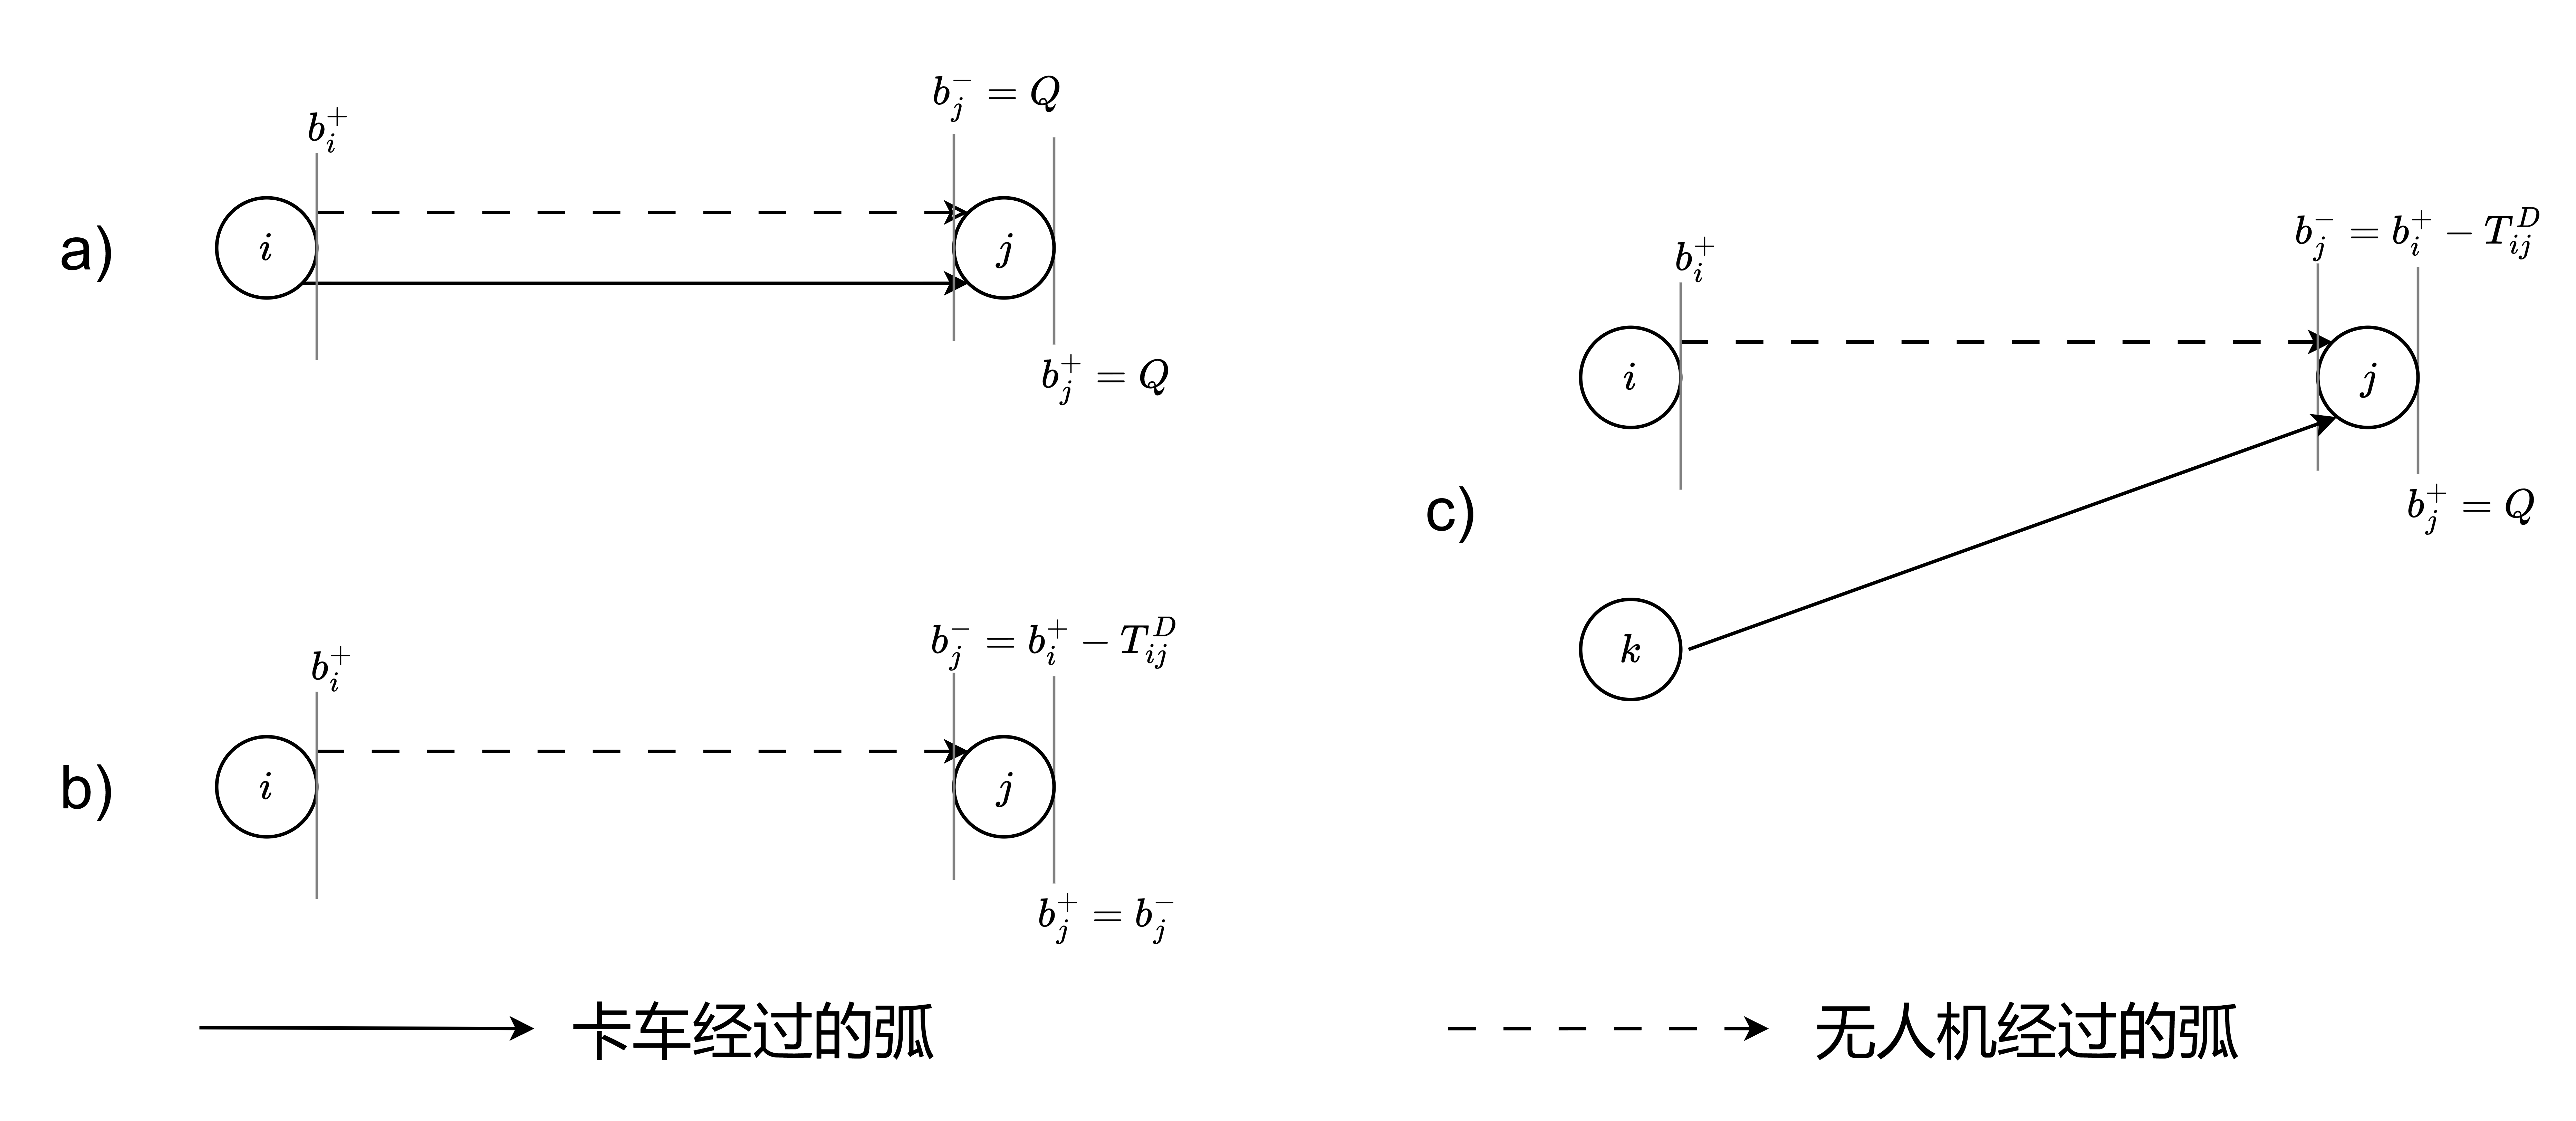
\includegraphics[width=\linewidth]{images/tdtl.drawio.png}\\
    \caption{TDTL模型无人机电量约束类型示意图}
    \label{fig:tdtl-drone-battery}
\end{figure}


Liu等(2021)\cite{liuTwoEchelonRoutingProblem2021}同样提出了类型为FSTSP-MD的MILP数学模型。在文章中作者称之为Two-Echelon Routing Problem for the Truck and Drone (2E-RP-T\&D)。但是不同于Gonzalez-R等(2020)\cite{gonzalez-rTruckdroneTeamLogistics2020}提出的TDTL模型,该问题考虑了不同重量的包裹对于无人机飞行消耗能源的影响。和FSTSP及TDTL一样,同样假设一辆卡车搭载一架无人机进行包裹递送,卡车的载重和续航没有进行限制,即卡车能够运送所有的包裹。该问题同样假设无人机和卡车在顾客点(或仓库)会合,但是该问题要求卡车必须先于无人机到达会合点(出于安全考虑)。2E-RP-T\&D的目标是最小化无人机和卡车的总成本。

% 关键假设如下:
%
% \begin{itemize}
%     \item 不考虑服务时间和无人机在顾客点的成本。
% \end{itemize}
%
% 2E-RP-T\&D数学模型的符号含义如表\ref{tab:2e-rp-td-sign-meaning}所示。
%
% \begin{table}[!htbp]
%     \centering
%     \caption{2E-RP-T\&D 模型符号及含义}
%     \label{tab:2e-rp-td-sign-meaning}
%     \begin{tabularx}{\textwidth}{lX}
%         \toprule[1pt]
%         符号 & 含义 \\
%         \midrule[0.75pt]
%         $G = (N, E)$ & 问题定义的无向图 \\
%         $N = V_{0} \cup V$ & 图 $G$ 的节点集合,其中 $V_{0} = \{0\}$ 表示仓库,$V = \{1, 2, \ldots, n\}$ 表示客户节点集合 \\
%         $E$ & 图 $G$ 中的链接集合,表示卡车或无人机可以行驶的路径 \\
%         $R$ & 卡车可以行驶的所有可能的有向主路线集合 \\
%         $E_r$ & 在有向主路线 $r$ 中的边集合,$r \in R$是卡车的一条有向主路线\\
%         $S_{r}$ & 在主路线 $r$ 中包含的所有子路线集合 \\
%         $l \in S_{r}$ & 主路线 $r$ 中的一条子路线 \\
%         $R_{r l}$ & 当卡车行驶子路线 $l$ 时,无人机可以行驶的所有可能的有向伴随子路线集合 \\
%         $m \in R_{r l}$ & 无人机的一条有向伴随子路线 \\
%         $V_{r}$ & 当卡车沿主路线 $r$ 行驶时,卡车访问的客户节点集合 \\
%         $V_{r}^{\prime}$ & 在主路线 $r$ 中需要由无人机服务的客户节点集合 \\
%         $V_{r l m}$ & 在主路线 $r$ 的子路线 $l$ 对应的伴随子路线 $m$ 中,无人机访问的客户节点集合 \\
%         $E_{r l m}$ & 在主路线 $r$ 的子路线 $l$ 对应的伴随子路线 $m$ 中包含的弧集合 \\
%         $t_{i j}$ & 从客户 (或仓库) $i$ 到客户 (或仓库) $j$ $(i, j \in V_{0} \cup V)$ 的卡车行驶时间。 \\
%         $t_{i j}^{D}$ & 从客户 (或仓库) $i$ 到客户 (或仓库) $j$ $(i, j \in V_{0} \cup V)$ 的无人机飞行时间。 \\
%         $d_{i j}$ & 从客户 (或仓库) $i$ 到客户 (或仓库) $j$ $(i, j \in V_{0} \cup V)$ 的行驶距离。 \\
%         $w_{i}$ & 需要交付给客户 $i$ 的包裹重量,其中 $i \in V$ \\
%         $w_{d}$ & 无人机自身的重量 \\
%         $W_{H}$ & 无人机的最大载重量 \\
%         $P$ & 无人机电量容量的最大值 \\
%         $TH$ & 无人机的最大续航时间。 \\
%         $G_{i}$ & 无人机离开客户 (或仓库) $i$ 时的载重量,其中 $i \in V \cup V_{0}$ \\
%         $v_{i j}$ & 无人机离开客户 (或仓库) $i$ 到客户 (或仓库) $j$ 时的飞行速度,其中 $i, j \in V_{0} \cup V$ \\
%         $c_r$ & 卡车在主路线 $r \in R$ 上行驶所花费的成本 \\ 
%         $c_{rlm}$ & 无人机在主路线 $r$ 的子路线 $l$ 对应的伴随子路线 $m$ 上行驶所花费的成本 \\  
%         $F_{i j}$ & 从客户 $i$ 到客户 $j$ $(i, j \in V_{0} \cup V)$ 的无人机飞行能耗。 \\
%         $p_{i}$ & 无人机到达节点 $i$ 时的电池电量。 \\
%         $p_{i}^{+}$ & 无人机离开节点 $i$ 时的电池电量。 \\
%         $x_{r}$ & 二元变量,如果卡车选择有向主路线 $r$ 行驶,则等于 1,否则为 0,其中 $r \in R$ \\
%         $y_{r l m}$ & 二元变量,如果无人机选择伴随子路线 $m$ 行驶,则等于 1,否则为 0,其中 $m \in R_{r l}, l \in S_{r}, r \in R$ \\
%         $a_{i j r l}$ & 二元参数,如果弧 $(i, j) \in E_{r l}$,则等于 1,否则为 0 \\
%         $b_{i r l m}$ & 二元参数,如果 $i \in V_{r l m}$,则等于 1,否则为 0 \\
%         \bottomrule[1pt]
%     \end{tabularx}
% \end{table}
%
% 2E-RP-T\&D数学模型可以表示为MILP \ref{model:model-2e-rp-td}。
%
% {
% \newcommand{\myYellowTag}[1]{\label{#1}\tag{\colorbox{shallow-yellow}{\theequation}}\addtocounter{equation}{1}}
% \newcommand{\myRedTag}[1]{\label{#1}\tag{\colorbox{shallow-red}{\theequation}}\addtocounter{equation}{1}}
% \newcommand{\myGreenTag}[1]{\label{#1}\tag{\colorbox{shallow-green}{\theequation}}\addtocounter{equation}{1}}
% \newcommand{\myPurpleTag}[1]{\label{#1}\tag{\colorbox{shallow-purple}{\theequation}}\addtocounter{equation}{1}}
% \newcommand{\myBlueTag}[1]{\label{#1}\tag{\colorbox{shallow-blue}{\theequation}}\addtocounter{equation}{1}}
%
% \begin{model}{2E-RP-T\&D MILP}{model-2e-rp-td}
% \begin{align}
%     \text{s.t.} \quad & \sum_{(i,j) \in E_{rlm}}F_{ij} \leq P, \quad \forall m \in R_{rl} \myRedTag{eq:2e-rp-td-drone-battery-limit}\\
%     \quad & \sum_{i \in V_{rlm}}w_i \leq W_H, \quad \forall m \in R_{rl} \myRedTag{eq:2e-rp-td-drone-payload-limit}\\
% \end{align}
% \end{model}
% }
%
%
% \begin{itemize}
%     \item \colorbox{shallow-red}{无人机相关的约束:}约束\ref{eq:2e-rp-td-drone-battery-limit}要求无人机在伴随子路径 $m$ 行驶过程的能源总消耗不超过无人机的总电量,约束\ref{eq:2e-rp-td-drone-payload-limit}要求无人机在伴随路径 $m$ 行驶过程中的运输包裹总重量不超过无人机的最大载重量。 
% \end{itemize}

Windras Mara等(2022)\cite{windrasmaraAdaptiveLargeNeighborhood2022}在Gonzalez-R等(2020)\cite{gonzalez-rTruckdroneTeamLogistics2020}的基础上提出了multi-drop FSTS,但是不同于Gonzalez-R等(2020)\cite{gonzalez-rTruckdroneTeamLogistics2020}的假设,该模型考虑了起飞和降落的服务时间。

multi-drop FSTSP数学模型的符号含义如表\ref{tab:multi-drop-fstsp-sign-meaning}所示。

\begin{table}[!htbp]
    \centering
    \caption{multi-drop FSTSP 数学模型符号及含义}
    \label{tab:multi-drop-fstsp-sign-meaning}
    \begin{tabularx}{\textwidth}{lX}
        \toprule[1pt]
        符号 & 含义 \\
        \midrule[0.75pt]
        $n$ & 顾客的数量\\ 
        $k$ &操作的索引\\ 
        $G = (V, A)$ & 定义了要访问的节点集合 $V$ 和连接它们的弧集合 $A$ 的图 \\
        $V$ & 图 $G$ 的节点集合,包括一个仓库节点 $\{0\}$ 和 $n$ 个客户节点 $N = \{1, 2, \dots, n\}$ \\
        $A$ & 图 $G$ 中的弧集合,连接节点对 $(i, j)$,其中 $i, j \in V$ \\
        $Vd \subseteq V$ & 可以由无人机服务的节点子集 \\
        $N$ & 客户节点集合,即 $N = \{1, 2, \dots, n\}$ \\
        $K = [OP_1, \cdots, OP_k]$ & 所有可行操作的集合 \\
        $C$ & 卡车路径的非负节点数组 \\
        $D$ & 无人机路径的非负节点数组 \\
        $S \subseteq V$ & 节点的子集\\ 
        $OP_{k} = \{\mathscr{T}_k,\mathscr{D}_k\}$ & 第$k$次递送的顺序,也被称为operation,其中 $\mathscr{T}_k$ 是卡车在 $OP_k$ 时必须访问的节点序列,$\mathscr{D}_k$ 是无人机在 $OP_k$ 时必须访问的节点序列 \\ 
        $K(v)$ & 包含了节点 $v$ 的所有可行操作集合\\ 
        $K^-(v)$ & 包含了以节点 $v$ 为起始点或发射点的所有可行操作集合\\ 
        $K^+(v)$ & 包含了以节点 $v$ 为终止点或会合点的所有可行操作集合\\ 
        $K^{\mathscr{T}}(v)$ & 包含了以卡车访问节点 $v$ 的所有可行操作集合\\ 
        $K^{\mathscr{D}}(v)$ & 包含了以无人机访问节点 $v$ 的所有可行操作集合\\ 
        $c_n$ & 顾客的需求\\ 
        $d_{i\to j}^\mathscr{T}$ & 卡车从节点 $i$ 行驶到 $j$ 的距离 \\ 
        $d_{i\to j}^\mathscr{D}$ & 无人机从节点 $i$ 行驶到 $j$ 的距离 \\ 
        $\tau_{i\to j}^\mathscr{T}$ & 弧 $(i, j) \in A$ 上卡车的行驶时间 \\
        $\tau_{i\to j}^\mathscr{D}$ & 弧 $(i, j) \in A$ 上无人机的行驶时间 \\
        $s^L$ & 无人机的启动时间 \\
        $s^R$ & 无人机的回收时间 \\
        $\epsilon$ & 无人机的续航时间 \\
        $w_r^{\mathscr{T}}$ & 卡车在节点 $j$ 的等待时间 \\
        $w_r^{\mathscr{D}}$ & 无人机在节点 $j$ 的等待时间 \\
        $t(\mathscr{T}_k)$ & 卡车在 $OP_k$ 中完成其对应任务所需的时间,计算公式为\ref{eq:multi-drop-fstsp-operation-time-2} \\
        $t(\mathscr{D}_k)$ & 无人机在 $OP_k$ 中完成其对应任务所需的时间,计算公式为\ref{eq:multi-drop-fstsp-operation-time-3} \\
        $t_k = t(OP_k)$ & $OP_k$ 的完成时间($OP_k$的成本函数),计算公式为\ref{eq:multi-drop-fstsp-operation-time-1} \\
        $x_k$ & 二元决策变量,如果选择操作$k$ ,则等于 1,否则等于 0 \\
        $Y_v$ & 二元辅助决策变量,如果节点 $v$ 被选为至少一个操作的起始节点,则等于 1,否则等于 0 \\
        \bottomrule[1pt]
    \end{tabularx}
\end{table}


\begin{definition}{time for operations}{definition-multi-drop-fstsp}
    \begin{align}
        t(OP_k) &= 
        \begin{cases}
            \max\{t(\mathscr{T}_k), t(\mathscr{D}_k)\}, & \text{当} OP_k \text{包含至少一个无人机访问的节点时} \\
            t(\mathscr{T}_k), & \text{其他}
        \end{cases}\label{eq:multi-drop-fstsp-operation-time-1}\\
        t(\mathscr{T}_k) &= 
        \begin{cases}
            s^L + \tau_{i \to C_1}^{\mathscr{T}} + \sum_{i=1}^{\lvert C\rvert - 1} \tau_{C_i \to C_{i+1}}^{\mathscr{T}} + \tau_{C_{\lvert C\rvert} \to j}^{\mathscr{T}} + s^R, & \text{当} D \neq \varnothing \text{且} \lvert C\rvert > 1 \\
            s^L + \tau_{i \to C_1}^{\mathscr{T}} + \tau_{C_1 \to j}^{\mathscr{T}} + s^R, & \text{当} D \neq \varnothing \text{且} \lvert C\rvert = 1 \\
            \tau_{i \to j}^{\mathscr{T}}, & \text{其他} 
        \end{cases}\label{eq:multi-drop-fstsp-operation-time-2}\\
        t(\mathscr{D}_k) &= 
        \begin{cases}
            s^L + \tau_{i \to D_1}^{\mathscr{D}} + \sum_{i=1}^{\lvert D\rvert -1} \tau_{D_i \to D_{i+1}}^{\mathscr{D}} + \tau_{D_{\lvert D\rvert} \to j}^{\mathscr{D}} + s^R, & \text{当} \lvert D\rvert > 1 \\
            s^L + \tau_{i \to D_1}^{\mathscr{D}} + \tau_{D_1 \to j}^{\mathscr{D}} + s^R, & \text{其他} 
        \end{cases}\label{eq:multi-drop-fstsp-operation-time-3}
    \end{align}
\end{definition}

multi-drop FSTSP 数学模型可以表示为MILP \ref{model:model-multi-drop-fstsp}。

{
\newcommand{\myYellowTag}[1]{\label{#1}\tag{\colorbox{shallow-yellow}{\theequation}}\addtocounter{equation}{1}}
\newcommand{\myRedTag}[1]{\label{#1}\tag{\colorbox{shallow-red}{\theequation}}\addtocounter{equation}{1}}
\newcommand{\myGreenTag}[1]{\label{#1}\tag{\colorbox{shallow-green}{\theequation}}\addtocounter{equation}{1}}
\newcommand{\myPurpleTag}[1]{\label{#1}\tag{\colorbox{shallow-purple}{\theequation}}\addtocounter{equation}{1}}
\newcommand{\myBlueTag}[1]{\label{#1}\tag{\colorbox{shallow-blue}{\theequation}}\addtocounter{equation}{1}}

\begin{model}{multi-drop FSTSP MILP}{model-multi-drop-fstsp}
\begin{align}
    \min \quad & M = \sum_{k \in K}t_kx_k \label{eq:multi-drop-fstsp-obj}\\
    \text{s.t.} \quad & \sum_{k \in K(v)}x_k \geq 1, \quad \forall v \in V \setminus \{0\}\myGreenTag{eq:multi-drop-fstsp-customer-visit}\\
    \quad & \sum_{k \in K^{\mathscr{D}}(v)}x_k \leq 1, \quad \forall v \in Vd \setminus \{0\}\myGreenTag{eq:multi-drop-fstsp-customer-visit-drone}\\
    \quad & \sum_{k \in K^{\mathscr{T}}(v)}x_k \leq 2\left( 1 - \sum_{k \in K^{\mathscr{D}}(v)}x_k \right), \quad \forall v \in Vd \setminus \{0\}\myGreenTag{eq:multi-drop-fstsp-customer-visit-limit}\\
    \quad & \sum_{k \in K^+(v)}x_k \leq n Y_v, \quad \forall v \in V\myGreenTag{eq:multi-drop-fstsp-start-end-limit}\\
    \quad & \sum_{k \in K^+(v)}x_k = \sum_{k \in K^-(v)}x_k, \quad \forall v \in V\myBlueTag{eq:multi-drop-fstsp-hamiltonian-1}\\
    \quad & \sum_{k \in K^+(S)}x_k \geq Y_v, \quad \forall S \subset V \setminus \{0\}, v \in S\myBlueTag{eq:multi-drop-fstsp-hamiltonian-2}\\
    \quad & \sum_{k \in K^+(0)}x_k \geq 1\myBlueTag{eq:multi-drop-fstsp-hamiltonian-3}\\
    \quad & \tau_{i \to D_1}^{\mathscr{D}} + \sum_{i = 1}^{\lvert D\rvert -1}\tau_{D_i \to D_{i+ 1}}^{\mathscr{D}} + \tau_{\lvert D\rvert \to j}^{\mathscr{D}} + w_r^{\mathscr{D}} \leq \epsilon \myRedTag{eq:multi-drop-fstsp-drone-battery-limit}\\
    \quad & Y_0 = 1\label{eq:multi-drop-fstsp-start}\\
    \quad & x_k \in \{0,1\}, \quad \forall k \in K\label{eq:multi-drop-fstsp-x-limit}\\
    \quad & Y_v \in \{0,1\}, \quad \forall v \in V\label{eq:multi-drop-fstsp-y-limit}
\end{align}
\end{model}
}

目标函数\ref{eq:multi-drop-fstsp-obj}旨在最小化总路径的完成时间。

\begin{itemize}
    \item \colorbox{shallow-green}{顾客相关的约束:}约束\ref{eq:multi-drop-fstsp-customer-visit}确保所有的节点都被至少访问过一次;约束\ref{eq:multi-drop-fstsp-customer-visit-drone}确保所有可以被无人机服务的顾客点最多被无人机服务一次;约束\ref{eq:multi-drop-fstsp-customer-visit-limit}确保被无人机服务过的节点不会被卡车服务,反之亦然,系数2是由于当无人机没有服务过节点 $v$ 时,节点 $v$ 可以作为卡车某个操作的终点及另一个操作的起点(即在节点$v$最多在两个操作中存在,一次作为操作的起点,一次作为操作的终点);约束\ref{eq:multi-drop-fstsp-start-end-limit}表示如果节点 $v$ 是某个操作的终止节点,那么节点 $v$ 一定要是某个操作的起始节点。 
    \item \colorbox{shallow-blue}{Hamilton 图\cite{HamiltonianPathWikiwand}约束:}约束\ref{eq:multi-drop-fstsp-hamiltonian-1}确保以节点 $v$ 为终止点的操作接下来的操作会以节点 $v$ 为起始点(流量平衡约束);约束\ref{eq:multi-drop-fstsp-hamiltonian-2}确保任何非空的客户子集$S$必须至少有一个操作从外部进入,即如果节点 $v$ 被选为某个操作的起始节点($Y_v = 1$),则必须存在至少一个操作进入包含$v$的子集$S$,避免子回路的产生(消除子回路约束);约束\ref{eq:multi-drop-fstsp-hamiltonian-3}确保终止点为仓库的操作只有一次,这是因为如果终止点为仓库的操作大于1次,由于约束\ref{eq:multi-drop-fstsp-customer-visit-limit}限制了卡车和无人机服务节点的次数,并且约束\ref{eq:multi-drop-fstsp-customer-visit}确保每个节点都被访问过至少一次,而目标函数是最小化时间成本,如果多次以仓库为终止点的操作存在,则会增加成本,因此终止节点为仓库的操作大于1次的情况会被过滤掉。
    \item \colorbox{shallow-red}{无人机相关的约束:}约束\ref{eq:multi-drop-fstsp-drone-battery-limit}要求无人机在一次sortie过程中消耗的电量不能超过其续航限制。
    \item 决策变量和辅助决策变量及初始值:约束\ref{eq:multi-drop-fstsp-start}通过确保仓库被作为起点访问使得仓库作为路径的起始点;约束\ref{eq:multi-drop-fstsp-x-limit}和\ref{eq:multi-drop-fstsp-y-limit}定义了决策变量 $x_k$ 和辅助决策变量 $Y_v$ 的取值范围。 
\end{itemize}

\section{Parallel Drone Scheduling Traveling Salesman Problem}

Parallel Drone Scheduling Traveling Salesman Problem (PDSTSP) 同样由Murray等(2015)\cite{murrayFlyingSidekickTraveling2015}提出。PDSTSP适用于大量的顾客节点在无人机直接从仓库起飞的续航里程范围内。PDSTSP描述:一辆卡车和一群(单个或者多个都可以)完全相同的无人机从单个仓库出发分别服务顾客,每个顾客只能被服务一次,卡车遵循TSP路径服务,无人机直接从仓库起飞服务顾客,不同于FSTSP,PDSTSP中的无人机不需要和卡车进行会合。PDSTSP的目标是最小化最终到达仓库的卡车(无人机)的时间。

PDSTSP数学模型的符号含义如表\ref{tab:pdstsp-sign-meaning},基本上沿用了FSTSP的符号。

\begin{table}[!htbp]
    \begin{threeparttable}
    \centering
    \caption{PDSTSP模型符号及含义}
    \label{tab:pdstsp-sign-meaning}
    \begin{tabularx}{\textwidth}{lX}
        \toprule[1pt] % 表头线宽1镑(point, pt)
        符号 & 含义 \\
        \midrule[0.75pt] % 表中间线宽0.75镑(point, pt)
        $0$ & 起点仓库 \\
        $c + 1$ & 终点仓库 \\
        $C=\{1,2,\cdots,c\}$ & 全部客户集合 \\
        $C' \subseteq C$ & 可以接受无人机访问的客户集合\hyperlink{tab:pdstsp-item-1}{\tnote{a}}\\
        $C'' \subseteq C'$ & 在无人机的航行范围内可以接受无人机服务的顾客集合\hyperlink{tab:pdstsp-item-2}{\tnote{b}}\\ 
        $N_0 = \{0,1,2,\cdots,c\}$ & 流出节点集合 \\
        $N_+ = \{1,2,\cdots,c + 1\}$ & 流入节点集合 \\
        $N = \{0,1,2,\cdots,c,c + 1\}$ & 全部节点集合 \\
        $v \in V$ & 无人机集合\\ 
        $\tau_{i,j}'/\tau_{i,j}$ & 弧$\langle i,j\rangle$的飞行/行驶时间成本 \\
        $1 \leq \hat{u}_i \leq c + 2$ & 卡车破子圈辅助变量 \\
        $\hat{y}_{i,v} \in \{0, 1\}, i \in C'', v\in V$ & 无人机访问决策变量\\ 
        $\hat{x}_{i,j} \in \{0, 1\}, i \in N_0, j \in \{N_+:j\neq i\}$ & 卡车路由决策变量\\ 
        \bottomrule[1pt] % 表尾线宽1镑(point, pt)
    \end{tabularx}
    \begin{tablenotes}
        \footnotesize % 设置脚注内容字体大小为\footnotesize
        \item[a] \hypertarget{tab:pdstsp-item-1}{}指包裹重量没有超过无人机的载重限制,不需要顾客签收,顾客的位置允许无人机起降等限制。
        \item[b] \hypertarget{tab:pdstsp-item-2}{}当$\tau_{0,i}'+\tau_{i,c+1}'\leq e$时,顾客$i \in C'$属于集合$C''$。
    \end{tablenotes}
    \end{threeparttable}
\end{table}
\hyperlink{tab:fstsp-item-4}{\tnote{d}}


PDSTSP数学模型可以表示为MILP \ref{model:model-pdstsp}。

{
\newcommand{\mySubstack}[1]{\mathclap{\substack{#1}}}

\begin{model}{PDSTSP MILP}{model-pdstsp}
\begin{align}
    \min \quad & z \label{eq:pdstsp-obj}\\
    \text{s.t.} \quad & z \geq \sum_{\substack{i \in N_0}} \sum_{\substack{j \in N_{+}\\ j\neq i}}\tau_{i,j}\hat{x}_{i,j} \label{eq:pdstsp-truck-min-time}\\
    \quad & z \geq \sum_{i \in C''}(\tau_{0,i}' + \tau_{i, c+1}')\hat{y}_{i,v},\quad \forall v \in V\label{eq:pdstsp-drone-min-time}\\
    \quad & \sum_{\substack{i \in N_0\\ i\neq j}}\hat{x}_{i,j} + \sum_{\substack{v \in V\\ j \in C''}}\hat{y}_{j,v} = 1, \quad \forall j \in C\label{eq:pdstsp-customer}\\
    \quad & \sum_{j \in N_{+}}\hat{x}_{0,j} = 1\label{eq:pdstsp-truck-start}\\
    \quad & \sum_{i \in N_0}\hat{x}_{i,c+1} = 1\label{eq:pdstsp-truck-end}\\
    \quad & \sum_{\substack{i \in N_0\\i \neq j}}\hat{x}_{i,j} = \sum_{\substack{k \in N_{+}\\ k\neq j}}\hat{x}_{j,k}, \quad \forall j \in C\label{eq:pdstsp-truck-flow}\\
    \quad & \hat{u}_i - \hat{u}_j + 1 \leq (c+2)(1 - \hat{x}_{i,j}), \quad \forall i \in C, j \in \{N_{+}:j \neq i\}\label{eq:pdstsp-mtz}\\
    \quad & 1 \leq \hat{u}_i \leq c+2, \quad \forall i \in N_{+}\label{eq:pdstsp-u-bound}\\
    \quad & \hat{x}_{i,j} \in \{0,1\},\quad \forall i \in N_0, j \in \{N_{+}: j\neq i\}\label{eq:pdstsp-x-bound}\\
    \quad & \hat{y}_{i,v} \in \{0,1\},\quad \forall i \in C'', v \in V\label{eq:pdstsp-y-bound}
\end{align}
\end{model}
}

目标函数\ref{eq:pdstsp-obj}追求最小化完工时间$z$,即无人机和卡车最晚到达终点仓库的时间,通过约束\ref{eq:pdstsp-truck-min-time}和\ref{eq:pdstsp-drone-min-time}分别限制卡车和无人机最晚到达终点仓库的时间来实现;约束\ref{eq:pdstsp-customer}确保了每个顾客能且只能被服务一次,服务可以由无人机或者卡车提供;约束\ref{eq:pdstsp-truck-start}和\ref{eq:pdstsp-truck-end}要求卡车必须从起点仓库$0$出发并返回终点仓库$c+1$一次,约束\ref{eq:pdstsp-truck-flow}要求卡车在中间的顾客节点满足流入和流出相等的流约束;约束\ref{eq:pdstsp-mtz}是MTZ形式的破子圈约束;约束\ref{eq:pdstsp-u-bound},\ref{eq:pdstsp-x-bound}和\ref{eq:pdstsp-y-bound}给出了决策变量和辅助决策变量的取值范围。

Ham(2018)\cite{hamIntegratedSchedulingMtruck2018}在PDSTSP的基础上提出了multi-truck, multi-drone, and multi-depot scheduling problem constrained by time-window, drop-pickup synchronization, and multi-visit, with the objective to minimize the maximum completion time over all tasks ($\text{PDSTSP}^{\text{+DP}}$),不同于PDSTSP,该问题考虑了无人机递送和收回货物的情况,即当无人机递送货物到顾客返回时,可以飞行到另一个需要退货的顾客节点进行回收货物以使无人机满载,从而满足退货的需求。另外,该问题还考虑了服务顾客的时间窗问题,即顾客需求有时间限制,并且可以在不同的时间段为同一个顾客服务。
